\section{四条透明色带的 RenderDoc 截帧}
测试用四条等宽色带代替叶片，左右两条应当可见，中间透明。先用同一个矩形写深度，清空目标，再独立执行主绘制。分别读取两次输出，就能查出哪一次留下了错误的轮廓。

\begin{figure}[H]\centering
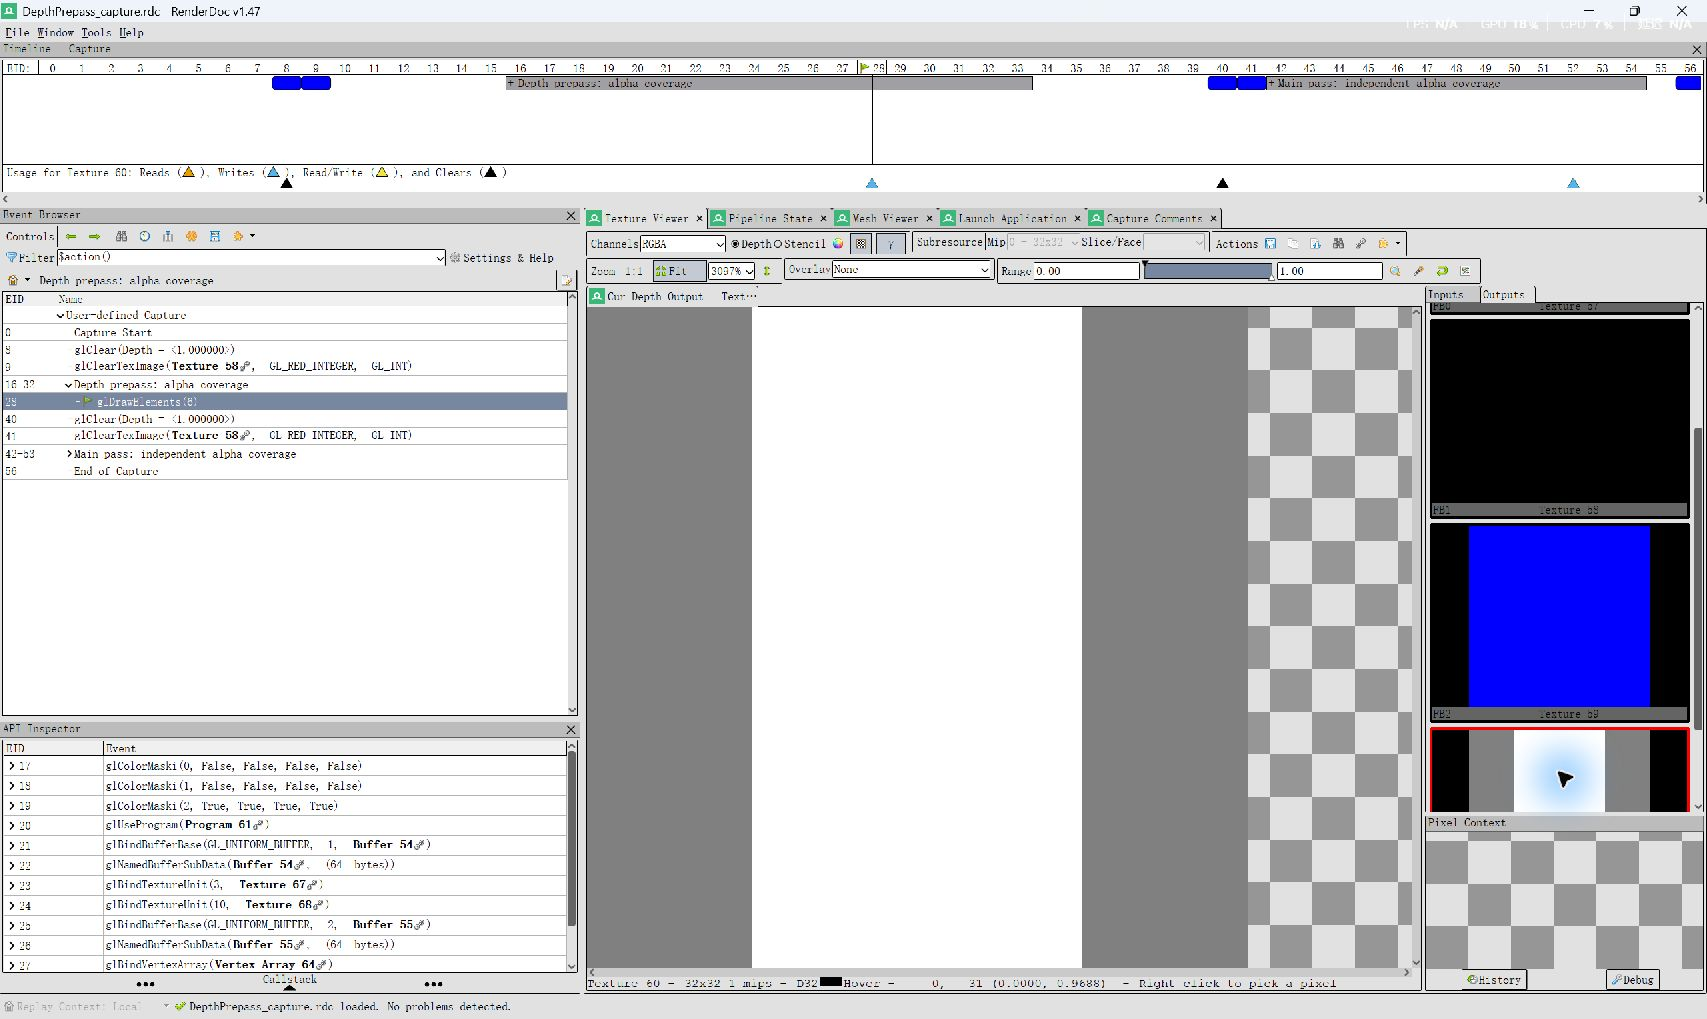
\includegraphics[width=.89\linewidth]{../../../output/captures/renderdoc-eid28-depth.jpg}
\caption{RenderDoc 1.47 回放窗口。事件 28 显示第一次绘制写入的深度图。沿左侧列表往下是清屏和主绘制，可切到事件 52 比较同一行像素。}
\end{figure}

\subsection{把材质透明度换算成预期像素}
回放显示，两次绘制使用的材质底色 alpha 都是 0.75，底色贴图与透明度贴图都已启用。Mask 阈值是 0.5。中左色带只有底色贴图变透明，中右色带只有透明度图变暗。两种来源单独作用，都应把透明度降到阈值以下。

\noindent\begin{tabularx}{\textwidth}{L{4.1cm}YYYY}
\toprule
输入与结果 & 左 & 中左 & 中右 & 右 \\
\midrule
底色贴图 alpha & 1 & $64/255$ & 1 & 1 \\
透明度贴图红通道 & 1 & 1 & $64/255$ & 1 \\
三项相乘后的 alpha & 0.75 & $\approx0.188$ & $\approx0.188$ & 0.75 \\
像素 & 保留 & 丢弃 & 丢弃 & 保留 \\
\bottomrule
\end{tabularx}

在 $32\times32$ 个像素上，两次绘制的深度逐字节相同。两侧共 512 个像素深度为 0.5，中间 512 个仍是清屏值 1.0。主绘制的实体编号也相应为 42 和 $-1$。这次捕获解释了相机所见的两次裁剪；光源看到的阴影与 RSM 轮廓另有逐像素测试。

在 RTX 5070 Ti Laptop GPU 上使用 RenderDoc 1.33 的 DLL 和 1.6.0 应用接口截帧，再用 1.47 回放。两次绘制各用六个索引。驱动在事件 28 报告顶点着色器因 OpenGL 状态重新编译，记录中没有给出重编译耗时或出现频率。
\note{原始帧、导出的两张深度图和像素读数保存在 \path{output/captures/}。运行 \path{tests/run_depth_tests.cmd} 可复现绘制，截帧参数见 \path{output/captures/README.md}。}
